\documentclass{standalone}
\usepackage{tikz}
\usepackage{ctex,siunitx}
\setCJKmainfont{Noto Serif CJK SC}
\usepackage{tkz-euclide}
\usepackage{amsmath}
\usetikzlibrary{patterns, calc}
\usetikzlibrary {decorations.pathmorphing, decorations.pathreplacing, decorations.shapes,}
\begin{document}
\small
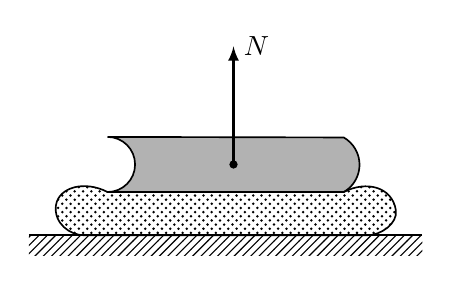
\begin{tikzpicture}[>=latex,scale=1]
  % \useasboundingbox(-1,-0.75)rectangle(3.7,1.4);
  \fill [fill=black!30, draw,semithick] (1,0.3)--(4,0.3)arc(-60:60:0.4)--(1,1)arc(90:-90:0.35)--cycle;
  \fill [pattern = north east lines] (0,-0.5) rectangle (5,-.25);
  \draw [thick](0,-0.25)--(5,-0.25);
  \draw[->,thick] (2.6,1.3/2)--(2.6, 1.3/2+1.5)node[right]{$N$};
  \fill (2.6,1.3/2) circle[radius=1.5pt];
  \fill [pattern = crosshatch dots,draw,semithick](1.000, 0.300)..controls(0.709, 0.451)and(0.382, 0.363)..(0.345, 0.133)..controls(0.313,-0.096)and(0.522,-0.250)..(0.708,-0.250)--(4.292,-0.250)..controls(4.478,-0.250)and(4.687,-0.096)..(4.662, 0.068)..controls(4.618, 0.363)and(4.291, 0.451)..(4.000, 0.300)--cycle
  ;
\end{tikzpicture}
\end{document}